% Figure from MATH 591 notes, section 15. Compile with the notes preamble.
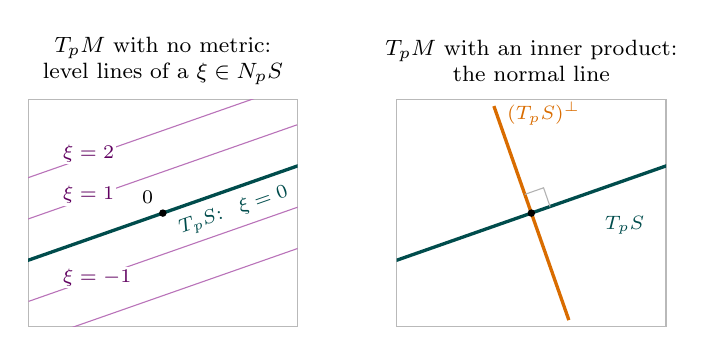
\begin{tikzpicture}[scale=0.9]
\draw[gray!55] (-1.90,-1.6) rectangle (1.90,1.6);
\node[font=\footnotesize, align=center] at (0.00,2.15){$T_pM$ with no metric:\\ level lines of a $\xi \in N_pS$};
\begin{scope}\clip (-1.9,-1.6) rectangle (1.9,1.6); \draw[violet!55] (-1.713,-1.765) -- (2.440,-0.311); \end{scope}
\begin{scope}\clip (-1.9,-1.6) rectangle (1.9,1.6); \draw[violet!55] (-1.895,-1.246) -- (2.258,0.208); \end{scope}
\begin{scope}\clip (-1.9,-1.6) rectangle (1.9,1.6); \draw[violet!55] (-2.258,-0.208) -- (1.895,1.246); \end{scope}
\begin{scope}\clip (-1.9,-1.6) rectangle (1.9,1.6); \draw[violet!55] (-2.440,0.311) -- (1.713,1.765); \end{scope}


\begin{scope}\clip (-1.9,-1.6) rectangle (1.9,1.6); \draw[teal!60!black, very thick] (-2.076,-0.727) -- (2.076,0.727); \end{scope}
\node[teal!60!black, font=\scriptsize, rotate=19.29] at (1.00,0.03) {$T_pS$: \ $\xi = 0$};
\fill (0,0) circle (1.5pt) node[above left, font=\scriptsize] {$0$};
\draw[gray!55] (3.30,-1.6) rectangle (7.10,1.6);
\node[font=\footnotesize, align=center] at (5.20,2.15){$T_pM$ with an inner product:\\ the normal line};
\begin{scope}\clip (3.30,-1.6) rectangle (7.10,1.6); \draw[teal!60!black, very thick] (3.124,-0.727) -- (7.276,0.727); \end{scope}
\draw[orange!85!black, very thick] (5.729,-1.510) -- (4.671,1.510);
\draw[gray!60] (5.464,0.092) -- (5.372,0.357) -- (5.108,0.264);
\node[teal!60!black, font=\scriptsize, anchor=north west] at (6.10,0.1) {$T_pS$};
\node[orange!85!black, font=\scriptsize, anchor=west] at (4.721,1.410) {$(T_pS)^\perp$};
\fill (5.20,0) circle (1.5pt);
\node[violet!75!black, font=\scriptsize, fill=white, inner sep=0.8pt, anchor=south west] at (-1.450,0.095) {$\xi = 1$};
\node[violet!75!black, font=\scriptsize, fill=white, inner sep=0.8pt, anchor=south west] at (-1.450,0.678) {$\xi = 2$};
\node[violet!75!black, font=\scriptsize, fill=white, inner sep=0.8pt, anchor=south west] at (-1.450,-1.070) {$\xi = -1$};
\end{tikzpicture}
